%!TEX root = Report.tex

\section{Tracking}
This chapter is divided into three subparts. First we will introduce the reader to different image processesing techniques, and their uses. Following this we will introduce the reader to a framework that supports these techniques, and finish off by describing the implemened solution and the design choices.

% Gå ud fra at dette afsnit ikke har noget video input fra et kamera. Integration med kameraet kommer senere.
% 
% Teori først - hvilken slags image manipulation har vi brugt? hvad var alternativerne?
% Så framework - vi bruger OpenCV, why? hvad giver det os? hvad er drawbacks?
% så implementation - Hvad har vi implementeret? Hvordan var performance? hvad var vores alternativer? har vi eksperiementeret med nogen af de andre muligheder?
% 
% Image Segmentation - hvad giver det os/hvorfor er det smart?
% Thresholding
% Dilating
% Eroding
% Background detection and why we can't use it
% Alternatives and why we don't use them

\subsection{Theory}
This section will provide information about five common image processing techniques; thresholding, dilating and eroding, image segmentation and background filtering. This information will be backed up by examples.

\subsubsection{Thresholding}
Thresholding is an image processing technique used to make a final decision about each pixel in an image. Either a pixel value is one that we are interested in or it is not. This is usually done by assigning a specific pixel value to the pixel we want, and another to those that we do not want. In general we compare the \textit{i}th pixel of the source image, \textit{src}, to the threshold value, \textit{T}, and saves the result in a destination image, \textit{dst}. For instance, to create a binary image where we are interested in all pixels above the threshold \textit{T}, the equation would look like show in Equation \ref{eq:binarythresholding},

\begin{equation}
dst_i = src_i \geq T ? 255: 0
\label{eq:binarythresholding}
\end{equation}

Most threshold operations are applied on grayscale images, where all pixel values range between 0 (black) and 255 (white). Sometimes these values are normalized to range between 0 and 1 instead. However for the rest of this report we will assume that grayscale images use the former convention. Soon we will argue how thresholding can be expanded to also cover thresholding an RGB image. Figure \ref{fig:threshold_example} show an example of applying threshold to a grayscale image.

\begin{figure}
        \centering
        \begin{subfigure}[b]{0.3\textwidth}
                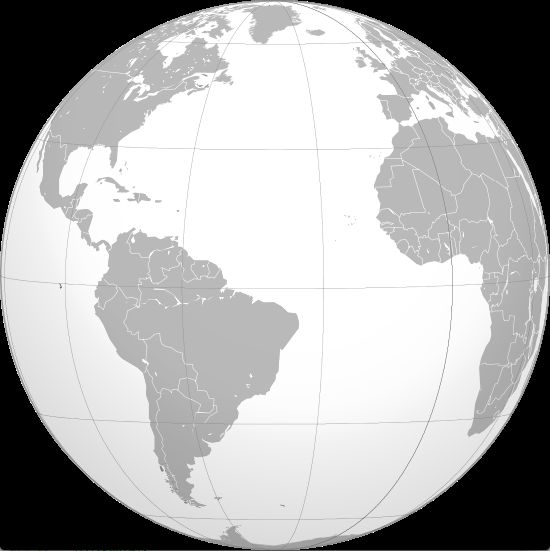
\includegraphics[scale = 0.2]{img/pre_threshold}
                \caption{Grayscale image}
        \end{subfigure}
		\quad
        \begin{subfigure}[b]{0.3\textwidth}
                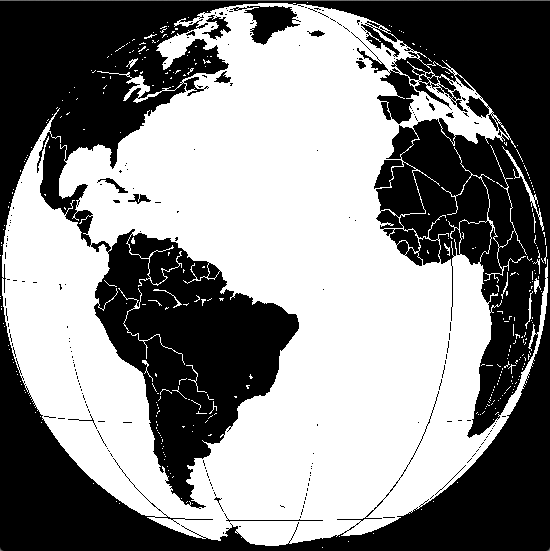
\includegraphics[scale = 0.2]{img/post_threshold}
                \caption{Thresholded image}
        \end{subfigure}
		\caption{An example of applying a threshold on a grayscale image. In this example with threshold value \textit{T} = 200}
		\label{fig:threshold_example}
\end{figure}

Now what happens if you what you are interested in is a color? To use thresholding we first need to convert it to a grayscale image. However doing so might provide an image that have lost important information as can be seen in figure \ref{fig:RGB2GRAY}. Unless you want to find the red color, you have no way of differentiating the blue and green color.

\begin{figure}
        \centering
        \begin{subfigure}[b]{0.3\textwidth}
                
\includegraphics[scale=0.5]{img/RGB}
                \caption{RGB image}
        \end{subfigure}
		\quad
        \begin{subfigure}[b]{0.3\textwidth}
                
\includegraphics[scale=0.5]{img/GrayRGB}
                \caption{Grayscale image}
        \end{subfigure}
		\caption{Example of grayscaling a color image}
		\label{fig:RGB2GRAY}
\end{figure}

A step in the right direction would be to define the threshold value \textit{T} as a scalar consisting of three values - one for each color channel. We will denote this threshold scalar as \textit{S} and define it as shown in Equation \ref{eq:thresholdscalar}.

\begin{equation}
S =  
\begin{pmatrix}
  S_{R}\\
  S_{G}\\
  S_{B}\\
\end{pmatrix}
\label{eq:thresholdscalar}
\end{equation}

To apply it to an RGB image we need to change Equation \ref{eq:binarythresholding} to the one shown in \ref{eq:threshold_RGB}.

\begin{equation}
{dst_i} = {src_i}_R \geq S_R \wedge {src_i}_G \geq S_G \wedge {src_i}_B \geq S_B? 255: 0
\label{eq:threshold_RGB}
\end{equation}

Trying it out makes it much easier to differentiate between colors. In Figure \ref{fig:RGB_Thresh} a threshold attemp using this method directly on the RGB image is shown.

\begin{figure}
        \centering
        \begin{subfigure}[b]{0.3\textwidth}
                
\includegraphics[scale=0.5]{img/RGB}
                \caption{RGB image}
        \end{subfigure}
		\quad
        \begin{subfigure}[b]{0.3\textwidth}
                
\includegraphics[scale=0.5]{img/RGBThresh}
                \caption{Thresholded image}
        \end{subfigure}
		\caption{Example of thresholding a color image with Equation \ref{eq:threshold_RGB} using the scalar \textit{S}=(0,100,0)}
		\label{fig:RGB_Thresh}
\end{figure}

\subsubsection{Dilating and Eroding}


\subsubsection{Image Segmentation}


\subsubsection{Background Filtering}


\subsection{Framework}
Something about opencv

\subsection{Realization}
Something about the solution


